\documentclass[11pt]{article}
\usepackage{amsmath, amsfonts, amsthm, amssymb}  % Some math symbols
\usepackage{enumerate}
\usepackage{fullpage}
\usepackage[x11names, rgb]{xcolor}
\usepackage{tikz}
\usepackage{graphicx}
\usetikzlibrary{snakes,arrows,shapes}
\usepackage{wasysym}
\usepackage{dsfont}
\usepackage{centernot}

\setlength{\parindent}{0pt}
\setlength{\parskip}{5pt plus 1pt}
\pagestyle{empty}

\def\indented#1{\list{}{}\item[]}
\let\indented=\endlist

\newcounter{questionCounter}
\newcounter{partCounter}[questionCounter]

\newenvironment{question}[2][\arabic{questionCounter}]{%
    \addtocounter{questionCounter}{1}%
    \setcounter{partCounter}{0}%
    \vspace{.25in} \hrule \vspace{0.5em}%
        \noindent{\bf #2}%
    \vspace{0.8em} \hrule \vspace{.10in}%
}{}

\renewenvironment{part}[1][\alph{partCounter}]{%
    \addtocounter{partCounter}{1}%
    \vspace{.10in}%
    \begin{indented}%
       {\bf (#1)} %
}{\end{indented}}

%%%%%%%%%%%%%%%%% Identifying Information %%%%%%%%%%%%%%%%%
%% This is here, so that you can make your homework look %%
%% pretty when you compile it.                           %%
%%     DO NOT PUT YOUR NAME ANYWHERE ELSE!!!!            %%
%%%%%%%%%%%%%%%%%%%%%%%%%%%%%%%%%%%%%%%%%%%%%%%%%%%%%%%%%%%
\newcommand{\myname}{Michael Rosenberg}
\newcommand{\myandrew}{mmrosenb@andrew.cmu.edu}
\newcommand{\mycourse}{73-449: Social, Economic, and Information Networks}
\newcommand{\myhwname}{| Final Project Proposal}
\newcommand{\myrecitation}{Anderson, Section A}
\newcommand{\myteammates}{}
\newcommand{\Z}{\mathds{Z}}
\newcommand{\bigdot}{\textbf{.} }
\newcommand{\spa}{\hspace{2cm}}
\newcommand{\proposition}{\textbf{\underline{Proposition:} }}
\newcommand{\proofwrite}{\textbf{\underline{Proof.} }}
\newcommand{\claim}{\textbf{\underline{Claim.} }}
\newcommand{\AFSOC}{Assume for the sake of contradiction }
\newcommand{\theorem}{\textbf{\underline{Theorem:}} }
\newcommand{\definition}{\textbf{\underline{Definition:}} }
\newcommand{\xNot}{\mathbf{x}_0}
%%%%%%%%%%%%%%%%%%%%%%%%%%%%%%%%%%%%%%%%%%%%%%%%%%%%%%%%%%%%%%%%%%%%%%%%%%%%%%%%

\begin{document}
\begin{center}
    {\Large \mycourse} {\Large \myhwname} \\
    \myrecitation \\
    \myname \\
    \myandrew \\
    %\myteammates 
\end{center}

For my final project, I will be doing an analysis of the Offshore Leaks
Database. This database shows relationships and networks among people and
companies in offshore entities that are traditionally designated as ``tax
havens''. Thus, to some degree, this database provides strong insights into how
the world's rich conduct offshore business. This database was constructed from
three leaks: the International Consortium of Investigative Journalists' (ICIJ)
China Leaks investigation in 2013, the Panama Papers leak in April 2016, and the
Bahamas Leak in September 2016.


\begin{figure}[h!]
    \centering
    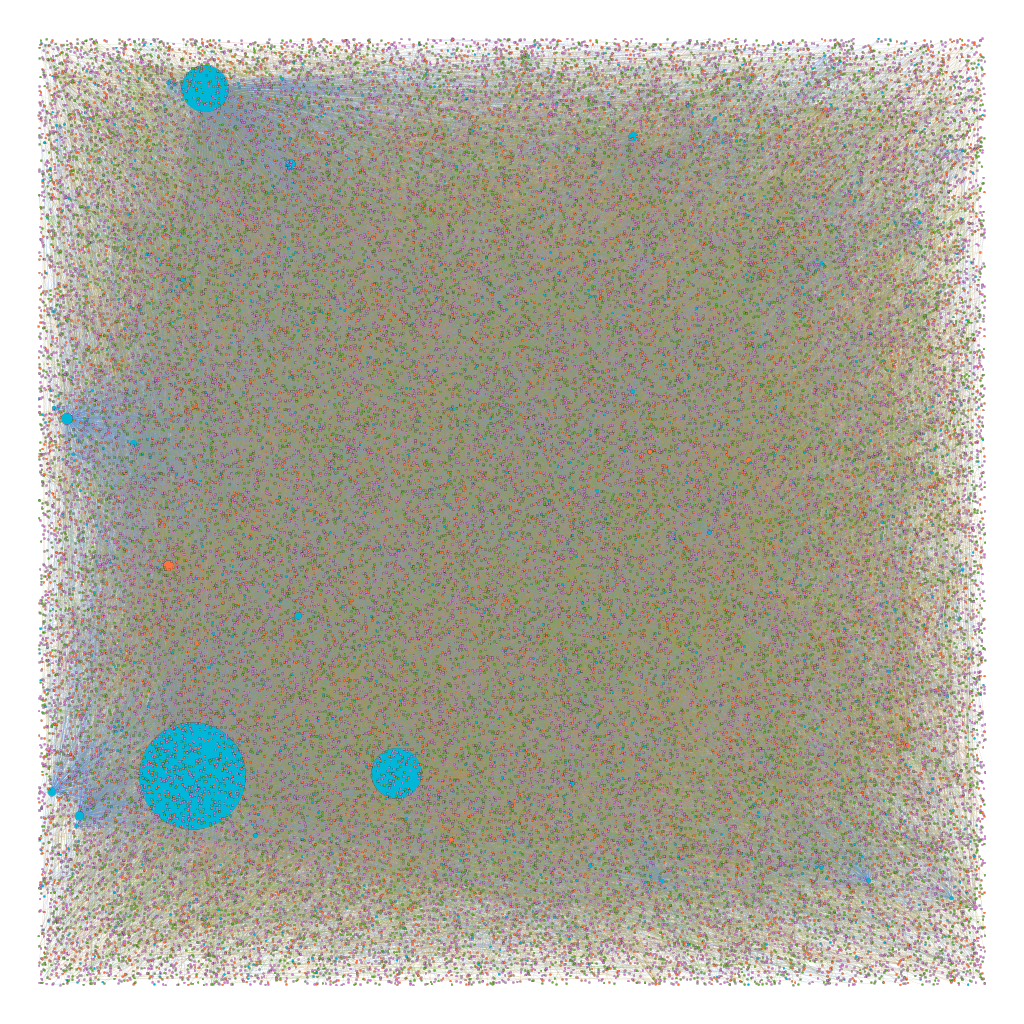
\includegraphics[width = 5in]{../analysis/figures/easternEuropeNetwork.png}
    \caption{Graph of our Eastern Europe network. The nodes are colored by
        agent type, where pink is for entities, green is for officers,
        orange is for addresses, and light blue is for intermediaries. Nodes
        are sized by degree.}
\end{figure}

\end{document}
